% ============================================================================
% paper9_v7_draft.tex --- Nature Sustainability skeleton draft
% ============================================================================
% Status: SKELETON. Abstract + Introduction + Results §1-7 + Discussion drafted
% from verified v6 + benchmark + toolbox numbers. Methods + Data/Code Availability
% + bibliography lifted as stubs from v6, to be polished separately.
%
% Decisions baked in (reasoned through with user 2026-05-18):
%   - Target: Nature Sustainability (primary). Backup: Nature Computational Science.
%   - Title: "Model-based AI planning enables county-scale farmland consolidation
%     in fragmented mountain landscapes"
%   - All abstract/intro/results numbers verified against v6.tex, benchmark
%     aggregate (105 + 42 JSONs), and toolbox memory; no fabricated data.
%   - Two open TODOs flagged inline: (a) [CITE: 7-deg threshold] in §2,
%     (b) toolbox 5-seed end-to-end vs 5-episode confirmation in §7.
%
% Source-of-truth numbers:
%   - Bishan (real): 13 townships, 2,600 blocks, 52,515 parcels, init slope
%     9.616 deg, init contiguity 3.585, 109 baimu fang totalling 46,844 ha.
%   - Neijiang (real): 29 townships, 3,711 blocks, 76,376 parcels, init slope
%     10.55 deg, init contiguity 2.63, 384 baimu fang totalling 74,342 ha.
%   - Bishan 5-seed contrastive MPC: -1.289% +/- 0.079% slope.
%   - Neijiang 5-seed from-scratch: -0.50% +/- 0.02% slope.
%   - Toolbox end-to-end (Bishan): -1.5439% +/- 0.0409% slope.
%   - Pairwise accuracy: 51.6% (MSE) -> 85.5% (lambda_rank=5.0).
%   - MPC ceiling: -0.209% +/- 0.008% (MSE-only).
%   - 7-preset benchmark: 27/35 cells at n=5, 4 partial, 4 missing PPO cells.
% ============================================================================

\documentclass[11pt]{article}

\usepackage{amsmath,amssymb}
\usepackage{booktabs}
\usepackage{graphicx}
\usepackage{multirow}
\usepackage{caption}
\usepackage{subcaption}
\usepackage{hyperref}
\usepackage{color}
\usepackage{natbib}
\usepackage[margin=1in]{geometry}
\usepackage{tikz}
\usetikzlibrary{positioning,arrows.meta,shapes.geometric,fit,backgrounds,calc}
\graphicspath{{./figures_v2/}}
\bibliographystyle{plainnat}

\newcommand{\todocite}[1]{\textcolor{red}{\textsuperscript{[CITE: #1]}}}

\begin{document}

\title{Model-based AI planning enables county-scale farmland consolidation in fragmented mountain landscapes}

\author{Ning Zhou$^{a,b,\ast}$\thanks{$^\ast$Corresponding author. \texttt{zhouning1@supermap.com}} and Xiang Jing$^{b}$\\
$^{a}${\em Public R\&D Center, SuperMap Software Co., Ltd., Beijing 100015, China}\\
$^{b}${\em School of Software and Microelectronics, Peking University, Beijing 100871, China}}

\date{}
\maketitle
\sloppy  % allow looser line breaks; prevents tech terms from overflowing right margin

% ============================================================================
\begin{abstract}
% ============================================================================
Land consolidation, the spatial rearrangement of farmland and forest parcels under regulatory and topographic constraints, raises productivity in fragmented mountain croplands but requires evaluating combinatorial trade-offs across tens of thousands of parcels at county scale, beyond the reach of manual planning or off-the-shelf artificial intelligence. Here we show that a single training-objective fix unlocks model-based reinforcement learning for this problem. Standard mean-squared-error training of a learned planning model masks a hidden ranking failure: per-action reward predictions are essentially random ($51.6\%$ pairwise accuracy), despite high aggregate fidelity ($0.998$ cosine similarity). An auxiliary pairwise large-margin loss raises ranking accuracy to $85.5\%$ and converts model-predictive control from failure to the strongest strategy we tested. On cadastral data from two southwest-China counties ($128{,}891$ parcels) and seven synthetic landscapes, the approach reduces farmland slope by 0.5 to 1.3$\%$ and forms larger mechanisable patches at two orders of magnitude lower compute than reinforcement-learning baselines. We release the benchmark and a deployable ArcGIS~Pro tool.
\end{abstract}

% ============================================================================
\section{Introduction}\label{sec:intro}
% ============================================================================

Mountainous and hilly landscapes contribute a substantial share of global agricultural production, but they pose management challenges distinct from those of the contiguous large fields of intensively farmed plains: small, irregular cadastral parcels are distributed across steep terrain \citep{romeo2020fao,liu2023fragmentation,foley2011solutions}. In these landscapes, parcel fragmentation has measurable consequences. It raises per-hectare labour cost, prevents the use of medium-scale agricultural machinery, increases vulnerability to climate-driven yield shocks, and limits the policy levers available for raising productivity without displacing farmers \citep{niu2023fragmentation,yu2020consolidation,springmann2018options,lambin2011global}. Land consolidation, the controlled spatial rearrangement of farmland and forest parcels within legal and topographic constraints, is the dominant policy response \citep{liu2014land,long2014rural,rounsevell2014challenges}. In China, where a substantial fraction of cultivated land lies in hilly or mountainous counties \citep{huang2018evaluation}, consolidation is operationalised through the formation of \textit{baimu fang} (literally ``hundred-\textit{mu} patches'', $\geq 6.67$\,ha of contiguous farmland) and through township-level regulatory plans that bound feasible swaps between farmland and forest classes \citep{liu2023fragmentation,rockstroem2009safe}.

Computationally, county-scale consolidation is a high-dimensional, multi-objective combinatorial planning problem: a single county routinely contains tens of thousands of parcels, three competing objectives (slope reduction for mechanisation, contiguity for shape, large-patch count for management), and hard adjacency and tenure constraints. Classical approaches range from rule-based greedy heuristics and metaheuristic optimisation such as genetic algorithms \citep{cao2012boundary,deb2002fast,stewart2004multi,aerts2002using,caoStewart2011integrated,ligmann2008integrating} to model-free deep reinforcement learning in related structured spatial settings \citep{zheng2023urban,equihua2024connectivity,janowicz2020geoai,sun2020optimal,verburg2008combined}. None of these scales cleanly to a county: heuristics ignore the multi-objective trade-off, metaheuristics miss long-horizon dependencies, and model-free reinforcement learning, in our experience, requires 8--12 GPU-hours per run and fails in 25--40\% of random seeds in the discrete county-scale regime, costs that effectively prevent iterative scenario exploration by planners.

Model-based reinforcement learning offers a structurally appealing alternative: learn the environment once from data, then exploit the learned dynamics for cheap planning \citep{chua2018deep,janner2019trust,nagabandi2018neural,kurutach2018model}. Recent work in continuous control \citep{hafner2025dreamerv3,hansen2024tdmpc2,hafner2019learning} and game-playing \citep{mnih2015human,silver2017mastering,vinyals2019grandmaster,wurman2022outracing} demonstrates the power of the paradigm, and learned-model planning underpins state-of-the-art performance in low-branching board games \citep{schrittwieser2020muzero}. AI-for-sustainability and Earth-observation work has begun to adopt these methods at policy scale \citep{rolnick2022tackling,reichstein2019deep,tuia2024artificial}. Yet for high-branching discrete spatial planning---the regime relevant to county-scale consolidation, factory job-shop scheduling, and combinatorial resource allocation---the question of \emph{whether learned models can plan reliably at all} has no clear answer. The existing benchmark literature is dominated by continuous-control or low-branching games, leaving the spatial-planning regime under-tested.

Here we show that the obstacle is not architectural but the training objective itself. We document a hidden ranking failure in standard mean-squared-error training of a county-scale world model: despite high aggregate accuracy (cosine similarity 0.998), per-action reward predictions are essentially random (pairwise accuracy 51.6\%), and this accounts for four independent failure modes we observe across dream-trained policies and model-predictive control on real cadastral data from Bishan District, Chongqing. We then show that adding an auxiliary pairwise large-margin ranking loss---an existing learning-to-rank technique \citep{burges2005learning,joachims2002optimizing,herbrich2000large}, applied here to the world model's reward head---closes this gap (pairwise accuracy 85.5\%) and converts model-predictive control from failure into the best-performing strategy. The same intervention generalises to a second county (Neijiang Dongxing District, Sichuan) and to seven synthetic stress-test landscapes spanning terrain, size, and fragmentation regimes. Beyond the empirical result, we release a deployable ArcGIS-Pro tool that lets county planners run the optimisation pipeline on their own data in minutes, and an open synthetic benchmark that lets the community compare future methods without access to sensitive cadastral data.

% ============================================================================
\section{Multi-objective consolidation as a planning problem at county scale}\label{sec:problem}
% ============================================================================

We anchor the analysis in two complete county-scale datasets from southwest China: Bishan District in Chongqing, and Neijiang Dongxing District in Sichuan. Both counties were obtained from the Third National Land Survey cadastral records and aggregate to a planning resolution that respects the township-level regulatory boundaries used in Chinese consolidation policy. Bishan covers 13 townships with 52{,}515 parcels grouped into 2{,}600 spatial blocks; Neijiang covers 29 townships with 76{,}376 parcels grouped into 3{,}711 blocks (Table~\ref{tab:counties}). The two counties together comprise 128{,}891 individual cadastral parcels, an order of magnitude larger than published consolidation benchmarks we are aware of \citep{cao2012boundary,zheng2023urban}.

The planning challenge is multi-objective and tightly coupled to terrain. The area-weighted mean farmland slope is $9.62^{\circ}$ in Bishan and $10.55^{\circ}$ in Neijiang, both above the $6^{\circ}$ terracing threshold of the Chinese High-Standard Farmland Construction standard (GB/T 30600-2022) beyond which mechanised cultivation requires terraced fields. The within-farmland contiguity index is 3.59 in Bishan and 2.63 in Neijiang, with the lower Neijiang value reflecting more aggressive fragmentation by ridges, water channels, and post-1980s smallholder boundaries. The legally relevant consolidation unit, the \textit{baimu fang} (literally ``hundred-\textit{mu} patch''; $\geq 6.67$\,ha of contiguous farmland eligible for mechanised management), is itself unevenly distributed: Bishan has 109 such patches in the initial state, totalling $46{,}844$\,ha, while Neijiang has 384 patches totalling $74{,}342$\,ha. A successful plan must reduce farmland slope, raise contiguity, and increase the count of qualifying \textit{baimu fang} patches simultaneously, under hard adjacency constraints (paired farmland--forest swaps) and a township-level swap budget that approximates the regulatory red line on total cultivated area.

\begin{table}[htbp]
\centering
\small
\caption{The two real-county datasets that anchor the cadastral evaluation. Both counties were extracted from the Third National Land Survey records and aggregated to spatial blocks (the planning units used by the model). Initial-state values are computed from the cadastral data before any optimisation. \textit{Baimu fang}: contiguous farmland patches of $\geq 6.67$\,ha (the legal threshold for mechanised consolidation eligibility under Chinese policy).}
\label{tab:counties}
\begin{tabular}{lcc}
\toprule
 & Bishan, Chongqing & Neijiang Dongxing, Sichuan \\
\midrule
Townships                                & 13       & 29       \\
Cadastral parcels                        & 52{,}515 & 76{,}376 \\
Spatial blocks (planning units)          & 2{,}600  & 3{,}711  \\
Initial farmland slope (deg)             & 9.62     & 10.55    \\
Initial contiguity index                 & 3.59     & 2.63     \\
Initial \textit{baimu fang} count        & 109      & 384      \\
Initial \textit{baimu fang} area (ha)    & 46{,}844 & 74{,}342 \\
\bottomrule
\end{tabular}
\end{table}

Three observations make this problem hard to attack with current methods. First, the action space is combinatorial: at each planning step the agent chooses one of 2{,}600 blocks (Bishan) or 3{,}711 blocks (Neijiang), and the environment then internally executes up to five paired farmland--forest swaps within that block under a deterministic feasibility rule (Methods, \S\ref{sec:methods-action}). Across a 100-step episode, the joint decision space is approximately $2600^{100}$ in Bishan alone---vastly larger than any standard combinatorial benchmark in the spatial-planning literature. Second, the objectives interact: slope-reducing swaps near fragment boundaries often retire marginal farmland from the largest existing patches, so a planner who optimises slope greedily can lose qualifying area; conversely, a planner who maximises \textit{baimu fang} count can degrade slope. Third, the practical constraint is wall-time. We measured the in-house model-free deep reinforcement learning baselines on the same task (Centralised PPO and a multi-agent variant; full configuration in Supplementary Material \S S1): both require $8$--$12$ GPU-hours of training per random seed, and Centralised PPO collapses on $2$/$5$ seeds in our runs. These costs make iterative scenario exploration---the workflow that consolidation planners actually need---impractical with off-the-shelf AI.

In short, the morphology of the two counties (steep, fragmented, multi-objective) and the cost profile of existing methods ($\sim$10 GPU-hours per scenario, with non-trivial failure rates) jointly define a gap that a purely architectural improvement cannot fill: even the best published model-free agent leaves the planner waiting hours for a single scenario, on a problem where the answer needs to be cheap enough to revisit dozens of times under different policy weightings. This is the gap we close in the remainder of the paper.

% ============================================================================
\section{Diagnosing a hidden ranking failure in the standard learned model}\label{sec:rank}
% ============================================================================

We trained a learned planning model---an ensemble of three transition networks, each with $\sim$237{,}000 parameters and the standard mean-squared-error reconstruction objective---on 6{,}000 transitions sampled from random and greedy policies in the Bishan environment. By the metrics conventionally used to declare a learned environment model ``good'', the result is unambiguously successful: state cosine similarity exceeds 0.998, training and validation losses converge cleanly, and the model is capable of being rolled forward autoregressively for 25 steps before its predictions begin to diverge perceptibly from the real environment ($s$-cosine drops from 0.999 at one step to 0.94 at 50 steps, and to 0.61 at 100 steps). Under any aggregate-fidelity test, this is a high-quality model.

The aggregate metrics, however, conceal a near-total failure of per-action discrimination. To isolate this, we constructed a pairwise-action benchmark: at each of 1{,}000 sampled environment states, we snapshotted the full simulator state, executed 50 valid actions one at a time, recorded the immediate ground-truth reward, and restored the snapshot before continuing. This dataset---50{,}000 ground-truth $(s, a, r)$ evaluations---lets us ask not ``does the model predict the right reward on average?'' but ``does the model rank actions in the right order at a given state?'' The answer is essentially no. The ground-truth pairwise standard deviation of reward across actions is $0.811$, but the MSE-trained ensemble predicts a standard deviation of only $0.274$---a three-fold compression of the discriminative signal. When we use the model to rank pairs of actions, it predicts the correct sign of the reward difference for only $51.6\%$ of pairs, statistically indistinguishable from random guessing.

The same gap appears at MPC inference time, when the model is asked to score 2{,}600 candidate blocks at a single environment state. The real-environment reward standard deviation across the 2{,}600 candidates is $1.5$, while the model's predicted reward standard deviation is $0.14$---a more than ten-fold underestimate. The model captures the mean of the action-conditioned reward distribution accurately but assigns nearly identical predicted rewards to actions whose true rewards differ by an order of magnitude. The standard ensemble disagreement diagnostic does not detect this failure: across 2{,}000 held-out on-policy transitions, Pearson correlation between ensemble reward standard deviation and absolute prediction error is $r = -0.024$ ($p = 0.29$). All five members of a 5-member ensemble converge to nearly identical predictions, and what little disagreement remains is initialisation noise, not epistemic uncertainty about which actions are good.

Four independent operational failures are explained by this hidden ranking gap. First, dream-trained policies become a coin-flip: under uncertainty-guided evidence collection, $99.6\%$ of candidate transitions are rejected by an ensemble-disagreement filter that carries no actual signal, dataset growth stalls at $6{,}017$ versus $8{,}000$ unfiltered, and slope improvement degrades from $-0.248\%$ to $-0.104\%$. Second, the random-sampling MPC ceiling is $-0.209\% \pm 0.008\%$ (Supplementary Table~S1), meaningful but well below the planner-relevant range. Third, every aggressive-exploitation variant fails: greedy continuation produces $+0.029\%$ (wrong direction) because a small positive bias in predicted reward leads the planner into trajectories that look good in the dream and are bad in reality; slope-only scoring yields $-0.001\%$ (effectively random action selection); value-guided terminal bonuses provide no improvement; doubling the candidate budget to $K{=}100$ gives no improvement either. Fourth, the failure is not removed by re-training: a fresh MSE-only ensemble of identical architecture and data reaches only $60.2\%$ pairwise ranking accuracy (Table~\ref{tab:contrastive-disc}), barely above the cached $51.6\%$ and far below the $85.5\%$ the auxiliary objective achieves at identical capacity. The missing ingredient is not in the architecture, the optimiser, or the random seed.

The diagnostic logic is now sharp. The model is not under-trained, under-parameterised, or starved of data: it has converged on a solution that minimises mean-squared error correctly. What it has not learned is the within-state ranking of actions, because mean-squared-error training places no penalty on assigning two actions the same predicted reward when their true rewards differ. In a high-branching discrete planning problem, this is exactly the wrong objective: every useful planning decision is a within-state ranking decision. Aggregate fidelity (cosine 0.998) and per-action discrimination (rank accuracy 51.6\%) are decoupled by construction, and standard model-evaluation metrics report the former while planning utility depends on the latter.

% MOVED TO SUPPLEMENTARY: tab:mpc-ablation (full ablation across continuation,
% scoring, terminal value, and search budget). Diagnostic numbers cited inline
% above already convey the failure pattern; the per-cell breakdown belongs in SI.

\begin{table}[htbp]
\centering
\small
\caption{Auxiliary contrastive training improves per-action discrimination without degrading aggregate fidelity. Predicted reward standard deviation is measured across 50 actions per state on held-out pairwise data. Ranking accuracy is the fraction of $1{,}000$ random action pairs where the model correctly predicts the sign of the reward difference. The true reward standard deviation across actions ($0.811$) bounds the recoverable signal. Even a fresh re-train with the same MSE-only objective ($\lambda_{\text{rank}}{=}0$) only reaches $60.2\%$ rank accuracy, confirming the failure is structural to the objective rather than to the optimiser.}
\label{tab:contrastive-disc}
\begin{tabular}{lcccc}
\toprule
Configuration & $\lambda_{\text{rank}}$ & Pred.\ reward std & Rank accuracy & Cos sim \\
\midrule
Baseline ensemble (MSE only, cached) & --- & $0.274$ & $0.516$ & $0.998$ \\
Retrained (MSE only)                  & $0.0$ & $0.715$ & $0.602$ & $0.9997$ \\
Contrastive (weak)                    & $1.0$ & $0.389$ & $0.816$ & $0.9997$ \\
\textbf{Contrastive (strong)}         & $\mathbf{5.0}$ & $0.183$ & $\mathbf{0.855}$ & $\mathbf{0.9991}$ \\
\midrule
True reward std (reference)           & --- & $0.811$ & --- & --- \\
\bottomrule
\end{tabular}
\end{table}

% ============================================================================
\section{Auxiliary ranking restores planning}\label{sec:fix}
% ============================================================================

The diagnosis points at a concrete intervention: add an explicit ranking signal to the model's reward head, applied at the same training stage as the existing reconstruction objective. We augment the standard mean-squared-error loss with a large-margin pairwise ranking term, following the classical learning-to-rank formulation \citep{herbrich2000large,joachims2002optimizing,burges2005learning,burges2010ranknet} that is conceptually related to representation-learning contrastive losses \citep{chen2020simple,oord2018representation}:
\begin{equation}
\mathcal{L} \;=\; \underbrace{\mathcal{L}_{\text{state}} + \mathcal{L}_{\text{global}} + 0.1\,\mathcal{L}_{\text{reward}}}_{\text{MSE terms}} \;+\; \lambda_{\text{rank}}\,\mathcal{L}_{\text{rank}}
\end{equation}
\begin{equation}
\mathcal{L}_{\text{rank}} \;=\; \mathbb{E}_{(s,a_i,a_j)\sim\mathcal{D}_{\text{pw}}}\!\left[\max\!\left(0,\; -\mathrm{sign}(r_i - r_j)\,(\hat{r}_i - \hat{r}_j) + m\right)\right]
\end{equation}
with margin $m{=}0.1$, chosen at approximately one-eighth of the empirical pairwise reward standard deviation ($0.811$); a coarse grid sweep of $m \in \{0.05, 0.1, 0.2\}$ on held-out validation showed a flat optimum (Methods, \S\ref{sec:methods-contrastive}). Two design choices are worth flagging. First, the auxiliary signal is applied to the world model's reward head, not to a separately learned reward proxy: the same network used for downstream planning is the one that learns to rank actions, so deployment requires no additional model. Second, this is a model-side, not a policy-side, use of pairwise preferences. The well-known RLHF formulation \citep{christiano2017deep,ouyang2022training} also uses pairwise comparisons, but to learn a reward function from human feedback that subsequently shapes a policy. We use pairwise comparisons to fix the ranking accuracy of an environment model that subsequently supports planning. The two usages share a mathematical form but operate at different points in the pipeline.

The training data are inexpensive to generate. We sample 1{,}000 environment states by random rollout, snapshot the simulator state at each, execute 50 valid actions one at a time, record the immediate ground-truth reward for each, and restore the snapshot before continuing. The result is a pairwise dataset $\mathcal{D}_{\text{pw}}$ of 50{,}000 ground-truth $(s, a, r)$ evaluations from which $\sim$1.2~million pairwise comparisons can be drawn. Generation took 45 minutes on commodity CPU hardware, of the same order as the $\sim$25\,min ensemble training cost. The procedure is simulator-specific in that it requires the ability to roll back state; in our cadastral simulator, this corresponds to caching the 19 environment attributes that fully determine a step. We discuss replay-buffer-based substitutes for environments without explicit snapshot/restore in the Discussion.

The intervention closes the discriminative gap with no measurable cost to aggregate fidelity (Table~\ref{tab:contrastive-disc}). Pairwise ranking accuracy rises from $60.2\%$ ($\lambda_{\text{rank}}{=}0$, MSE-only retrain) to $81.6\%$ ($\lambda_{\text{rank}}{=}1.0$) to $85.5\%$ ($\lambda_{\text{rank}}{=}5.0$), while state-prediction cosine similarity stays above $0.999$. Predicted reward standard deviation decreases from $0.715$ to $0.183$ as $\lambda$ grows: a margin loss penalises only incorrect ordering, not magnitude, and the model is free to satisfy it by compressing its outputs around a correct rank order. For planning, what matters is rank order, and the rank order is now correct on $85.5\%$ of pairs.

The qualitative effect on MPC is a reversal. With the MSE-only ensemble, the four variants tested in Section~\ref{sec:rank} all failed; with the contrastive ensemble at $\lambda_{\text{rank}}{=}5.0$, greedy continuation, the variant most cleanly attributed to ranking error, becomes the best (Table~\ref{tab:contrastive-mpc}). To establish that this is a property of the intervention rather than a single favourable run, we replicate across five independently trained ensembles. Cross-seed mean slope improvement is $-1.289\% \pm 0.079\%$, an approximately six-fold improvement over the previous MPC ceiling. A one-sample $t$-test against the fixed $-0.209\%$ baseline gives $t{=}{-27.3}$, $\mathrm{df}{=}4$, $p{=}1.07\times10^{-5}$. We caution against over-interpreting the effect size: the baseline standard deviation is episode-level while our replication standard deviation is cross-seed, a more conservative denominator. The substantive point is the qualitative shift, not the magnitude.

\begin{table}[htbp]
\centering
\small
\caption{MPC evaluation with contrastive-trained ensembles on the real Bishan environment ($H{=}5$, $K{=}50$). Rows for $\lambda \in \{0, 1.0\}$ and the $\lambda{=}5.0$ random row report episode-level standard deviation from a single ensemble (3 members). The starred $\lambda{=}5.0$ greedy row reports cross-seed mean $\pm$ standard deviation across 5 independently trained ensembles. Best overall in bold.}
\label{tab:contrastive-mpc}
\begin{tabular}{llccc}
\toprule
$\lambda_{\text{rank}}$ & Continuation & Slope \% & vs.\ baseline & Status \\
\midrule
0.0 (MSE only) & random & $-0.291 \pm 0.020$ & $-0.082$ & marginal \\
0.0 (MSE only) & greedy  & $-0.252 \pm 0.007$ & $-0.042$ & marginal \\
\midrule
1.0 & random & $-1.310 \pm 0.033$ & $-1.101$ & strong \\
1.0 & greedy & $-1.376 \pm 0.010$ & $-1.167$ & strong \\
\midrule
\textbf{5.0} & random & $\mathbf{-1.344 \pm 0.049}$ & $-1.135$ & \textbf{best random} \\
\textbf{5.0}$^\star$ & \textbf{greedy} & $\mathbf{-1.289 \pm 0.079}$ & $\mathbf{-1.080}$ & \textbf{best overall (5 seeds)} \\
\midrule
Baseline (MSE only, ceiling) & random & $-0.209 \pm 0.008$ & --- & reference \\
Baseline (MSE only)          & greedy & $+0.029 \pm 0.005$ & $+0.238$ & catastrophic \\
\bottomrule
\end{tabular}
\end{table}

% ============================================================================
\section{Real-county deployment: Bishan and Neijiang}\label{sec:counties}
% ============================================================================

The clearest test of the intervention is whether it produces planning outcomes that a county consolidation officer would recognise as useful, on the actual cadastral data the officer would supply. We deployed the contrastive-MPC pipeline end-to-end on Bishan District, Chongqing (52{,}515 parcels, 2{,}600 blocks), evaluating five independently trained ensembles for 100 planning steps each (one episode per ensemble). The outcomes are reported per seed in Table~\ref{tab:contrastive-multiobj} and aggregated as cross-seed mean $\pm$ standard deviation.

All three policy-relevant objectives move in the intended direction simultaneously. Area-weighted mean farmland slope decreases by $1.289\% \pm 0.079\%$ relative to the initial $9.62^{\circ}$ (CV $\approx 6\%$ across seeds), within-farmland contiguity rises by $0.0160 \pm 0.0016$, and the count of qualifying \textit{baimu fang} ($\geq 6.67$\,ha contiguous farmland units) increases by $+3.4 \pm 1.0$ relative to the initial 109 patches (Bishan baseline). One axis moves against the planner: total \textit{baimu fang} area decreases by $-312 \pm 34$\,ha, equivalent to $0.67\%$ of the initial $46{,}844$\,ha qualifying stock. This trade-off is intentional rather than incidental. Slope-reducing swaps disproportionately retire marginal farmland from the largest existing patches, while the count and contiguity reward terms pull the remaining area toward more compact configurations. The net planning effect---more qualifying large patches, lower total qualifying area, higher contiguity---matches the morphological intent of Chinese consolidation policy, where the regulatory constraint on absolute farmland area is enforced by a separate ``red line'' mechanism that our paired farmland--forest swap respects by construction (Methods, \S\ref{sec:methods-action}).

\begin{table}[htbp]
\centering
\small
\caption{Full multi-objective profile of contrastive MPC ($\lambda_{\text{rank}}{=}5.0$, greedy, $H{=}5$, $K{=}50$) on Bishan District across 5 independently trained ensembles (1 episode each). Initial state: slope 9.616, contiguity 3.585, 109 \textit{baimu fang} totalling 46{,}844\,ha. Slope and contiguity changes are both directionally correct. The count of large patches ($\geq$6.67\,ha) increases by $+3.4$ on average; total qualifying area decreases by $\sim$$312$\,ha because the agent consolidates many small patches into a smaller number of larger, contiguous patches---a deliberate trade-off discussed in \S\ref{sec:discussion}.}
\label{tab:contrastive-multiobj}
\begin{tabular}{ccccc}
\toprule
Seed & Slope \% & $\Delta$Contiguity & $\Delta$Baimu \# & $\Delta$Baimu (ha) \\
\midrule
0 & $-1.4235$ & $+0.0150$ & $+3$ & $-324.9$ \\
1 & $-1.2668$ & $+0.0165$ & $+3$ & $-283.6$ \\
2 & $-1.3250$ & $+0.0159$ & $+2$ & $-372.7$ \\
3 & $-1.2264$ & $+0.0139$ & $+5$ & $-278.2$ \\
4 & $-1.2018$ & $+0.0186$ & $+4$ & $-301.9$ \\
\midrule
\textbf{Mean} & $\mathbf{-1.289 \pm 0.079}$ & $\mathbf{+0.0160 \pm 0.0016}$ & $\mathbf{+3.4 \pm 1.0}$ & $\mathbf{-312.2 \pm 34.3}$ \\
\bottomrule
\end{tabular}
\end{table}

The intervention is competitive with model-free reinforcement-learning baselines we ran on the same task (Centralised PPO and a multi-agent variant; see Supplementary Material \S S1 for full configuration). Slope improvement under contrastive MPC ($-1.289 \pm 0.079\%$) is approximately $1.6\times$ larger than the multi-agent baseline ($-0.81 \pm 0.09\%$) and Centralised PPO baseline ($-0.79 \pm 0.36\%$), with comparable contiguity ($+0.016$) and \textit{baimu fang} count ($+3.4$ versus $+3.2$ and $+2.9$). Cross-seed slope variance is $4.6\times$ smaller than Centralised PPO and equal to MARL's, indicating consistent rather than lucky behaviour. The total qualifying-area loss is larger ($-312$\,ha versus $-75$ to $-97$\,ha), an honestly reported trade-off whose policy interpretation we return to in the Discussion. The cost asymmetry is the substantive deployment headline: the contrastive ensemble trains in 25 minutes on a commodity 12-thread CPU and runs each 100-step planning episode in approximately 225 seconds, against $8$--$12$ GPU-hours per seed for the in-house DRL baselines. The end-to-end wall-clock difference, on the same task and the same multi-objective reward, is roughly two orders of magnitude.

To test whether the intervention generalises beyond Bishan, we applied the full pipeline to Neijiang Dongxing District in Sichuan, a second county with 29 townships, 3{,}711 spatial blocks, and 76{,}376 cadastral parcels, larger and more fragmented than Bishan (contiguity $2.63$ versus $3.59$). Five seeds were run from scratch (regenerating both pairwise data and the transition model). The qualitative result holds: slope decreases by $0.50\% \pm 0.02\%$, contiguity rises by $0.034 \pm 0.001$, and the \textit{baimu fang} area trade-off flips sign to a $+267 \pm 38$\,ha gain. Three differences from Bishan emerge. Slope improvement is roughly half, consistent with Neijiang's flatter mean terrain leaving less slope-reduction headroom. Contiguity improvement is roughly twice as large, consistent with the more fragmented start. The area trade-off direction reverses: the agent gains rather than loses \textit{baimu fang} area because consolidation operates primarily on small fragments rather than retiring patches from the largest existing ones. Cross-seed slope standard deviation ($\pm 0.02\%$) is an order of magnitude smaller than the Bishan in-house DRL baselines, indicating clean cross-county stability.

A partial-transfer setting (Bishan-trained backbone, 5-episode local fine-tune) reaches similar slope ($-0.49 \pm 0.02\%$) but with degraded contiguity ($+0.024 \pm 0.003$) and a smaller, noisier area gain ($+62 \pm 80$\,ha). The Bishan-trained pairwise head appears to encode regional priors around slope gradients that do not transfer cleanly to flatter terrain; the recommended protocol on a new county is therefore to re-run the $\sim$45-minute pairwise pipeline locally, treating partial transfer as a warm-start heuristic only when pairwise data are scarce.

\paragraph{Robustness of the headline numbers.} Four independent verification layers underwrite the Bishan and Neijiang results above. (i)~A direct GIS recomputation from the optimised cadastral shapefile written to disk reproduces the slope, contiguity, and \textit{baimu fang} deltas to floating-point noise without invoking the learned ensemble (\S\ref{sec:methods-validate}); the headline gain is therefore a property of the on-disk geometry, not of the learned dynamics. (ii)~The contrastive ensemble's 1-step prediction error is measured directly against the true environment along the same 100-step trajectory MPC visits (\S\ref{sec:methods-mae}); the ensemble is mis-calibrated as a regressor (reward MAE $0.82$ against $\sigma(r_{\text{true}})=1.40$) yet recovers a Spearman rank correlation of $+0.22$ that is sufficient at H$=$5 horizon to reproduce the action sequence to floating-point identity, providing direct empirical support for the ranking-versus-regression decomposition of \S\ref{sec:rank}--\ref{sec:fix}. (iii)~A counter-factual ablation that replaces the ensemble entirely with the true \texttt{env.step} inside the scoring loop returns a slope of $-1.819\%$ in 358\,s of wall time, strictly worse on all three objectives than the ensemble pipeline's $-2.001\%$ in 1{,}448\,s; the ensemble's contribution to the result is therefore structural (full-action stage-1 coverage and cheap greedy continuation) rather than illusory (\S\ref{sec:methods-trueenv}). (iv)~Cross-county replication on Neijiang shows the qualitative result (slope down, contiguity up, low cross-seed variance) survives a 1.4$\times$ scale-up and a different morphology. Reviewers can rerun (i) end-to-end from the released shapefile and the released script in under two minutes; (ii) and (iii) reproduce in $\sim$25 and $\sim$6 minutes respectively on a desktop CPU.

% ============================================================================
\section{Cross-landscape stress test on a synthetic benchmark}\label{sec:bench}
% ============================================================================

The two-county evidence in Section~\ref{sec:counties} leaves open whether the result depends on properties shared by Bishan and Neijiang, both situated in southwestern hilly terrain. To test the method outside that regime, we constructed a synthetic benchmark of seven parametric landscapes varying along three morphological axes: terrain (hilly, mixed, plain), problem size (800, 2{,}600, 4{,}500 blocks), and fragmentation (consolidated, fragmented). Two presets (\texttt{bishan\_clone} and \texttt{neijiang\_clone}) are calibrated against the real anchors within the tolerance documented in Methods (\S\ref{sec:methods-synth}); the remaining five (\texttt{plain\_small\_cons}, \texttt{plain\_large\_cons}, \texttt{plain\_medium\_frag}, \texttt{mixed\_medium\_frag}, \texttt{hilly\_small\_cons}) are parameter-controlled stress tests rather than claims of regional generalisation. Each method runs for a 50-pair swap budget, one-tenth of the real-data episode length, to keep the per-cell wall-clock budget tractable across 175 cells. Only the relative ordering of methods, not absolute improvement magnitude, is intended to be comparable across the two evaluation regimes.

All seven landscapes are released as a public dataset (\S Data Availability), with the deterministic generator and a loader that exposes the synthetic states to the same simulator API used for real-data experiments. External researchers can reproduce our experiments and benchmark future methods without access to the sensitive Third National Land Survey records.

We benchmark five methods on the seven landscapes with five random seeds each: a uniform-random block selector, a slope-greedy heuristic, a genetic algorithm tuned for spatial layout problems \citep{cao2012boundary}, a centralised-PPO agent matching our model-free baseline, and the contrastive-MPC pipeline of Sections~\ref{sec:rank}--\ref{sec:counties}. All 175 cells (5 methods $\times$ 7 presets $\times$ 5 seeds) completed end-to-end. Slope improvements are reported in Table~\ref{tab:bench-slope}; $\Delta$contiguity, $\Delta$\textit{baimu fang} count, and area are reported in the Supplementary Material. Three patterns emerge.

First, on the five presets that are large or fragmented enough to make multi-step planning informative (\texttt{plain\_large\_cons}, \texttt{plain\_medium\_frag}, \texttt{mixed\_medium\_frag}, and the two real-data clones), contrastive MPC is the strongest method, with model-free PPO the consistent runner-up. The MPC slope-improvement margin over the genetic algorithm is $37.2\%$ on \texttt{plain\_large\_cons}, $23.7\%$ on \texttt{plain\_medium\_frag}, $6.4\%$ on \texttt{mixed\_medium\_frag}, $53.8\%$ on \texttt{neijiang\_clone}, and $48.3\%$ on \texttt{bishan\_clone} (full numbers in Table~\ref{tab:bench-slope}). On the small \texttt{hilly\_small\_cons} preset MPC also wins ($-0.271\%$ vs.\ GA $-0.295\%$, both close to the slope floor of the landscape). PPO ranks second on each of these six presets, never reaching MPC's slope despite comparable wall time. Absolute magnitudes are smaller than in the real-data results because synthetic episodes are an order of magnitude shorter. Cross-seed standard deviation for contrastive MPC is among the smallest of the five methods, indicating consistent rather than lucky behaviour.

Second, the one preset where contrastive MPC is \emph{not} dominant has a clean structural interpretation: it is small (800 blocks) and consolidated, leaving little headroom for sequential planning. On \texttt{plain\_small\_cons}, the genetic algorithm achieves $-2.757 \pm 0.203\%$, exceeding MPC's $-2.226 \pm 0.220\%$ and PPO's $-2.234 \pm 0.264\%$. The problem is small enough that GA's population-based exploration covers it within its 500-generation budget, while the planning value of contrastive ranking, which scales with the within-state action menu, is correspondingly muted. The crossover is consistent with the broader observation that learning-based planners need a sufficiently combinatorial action space to recoup their training cost.

Third, the wall-time profile reverses with problem size in a policy-relevant way. On the smallest preset (\texttt{plain\_small\_cons}, 800 blocks), GA finishes one seed in $\sim$67\,s versus MPC's $\sim$2.2\,h; on the largest (\texttt{plain\_large\_cons}, 4{,}500 blocks), GA needs $\sim$248\,s while MPC consumes $\sim$9.3\,h. Absolute time scales with problem size for both methods, but the planning-quality gap (Table~\ref{tab:bench-slope}) widens monotonically. PPO consumes wall time of order $\sim$0.5--1.5$\times$ MPC on every preset, never matching MPC's slope on the five planning-favourable presets. For a planner whose decision unit is the county, the relevant comparison is not which method is faster on a small toy but which scales without re-tuning to the deployed county's size and morphology; contrastive MPC delivers consistent slope improvement across 800--4{,}500 blocks under fixed hyperparameters, while GA's relative position degrades as problems grow.

One caveat qualifies the synthetic benchmark: the generator's calibration is verified to within $\pm 50\%$ on each axis for the two real-data clones; contiguity is the weakest axis (Bishan $\sim$$6\%$ deviation, Neijiang $\sim$$44\%$), reflecting Voronoi-based synthetic geometries' tendency to be more uniformly contiguous than real cadastre shaped by ridges, roads, and water channels. We flag this as a calibration limitation rather than a confound in the contrastive-MPC findings, which agree across synthetic and real regimes.

\begin{table}[htbp]
\centering
\small
\caption{Slope-improvement profile of five methods across the seven synthetic landscapes, $n{=}5$ seeds per cell (175 cells total). Values are mean $\pm$ sample standard deviation of the relative slope change in percent (negative is better). The rightmost column reports median wall-time per cell (seconds for fast methods, hours for learning-based). Best mean per row in bold. Contrastive MPC is the strongest method on the five planning-favourable presets (the two real-data clones and the three medium--large fragmented presets); the genetic algorithm wins on \texttt{plain\_small\_cons}, where the small action space lets a population search cover the optimum within budget. Numbers regenerated from \texttt{benchmark/results/} via \texttt{scripts/aggregate\_results.py}.}
\label{tab:bench-slope}
\resizebox{\textwidth}{!}{%
\begin{tabular}{lccccc@{\hspace{1.5em}}c}
\toprule
Preset & Random & Greedy & GA & PPO & MPC & Wall \\
($n_{\text{blocks}}$) & & & & & & (MPC) \\
\midrule
\texttt{bishan\_clone} (2{,}600)        & $-0.026{\pm}0.003$ & $-0.052{\pm}0.009$ & $-0.060{\pm}0.009$ & $-0.074{\pm}0.015$ & $\mathbf{-0.089{\pm}0.014}$ & $4.1$h \\
\texttt{neijiang\_clone} (3{,}700)      & $-0.011{\pm}0.002$ & $-0.025{\pm}0.004$ & $-0.026{\pm}0.005$ & $-0.036{\pm}0.011$ & $\mathbf{-0.040{\pm}0.007}$ & $6.1$h \\
\texttt{plain\_small\_cons} (800)        & $-0.544{\pm}0.072$ & $-0.996{\pm}0.268$ & $\mathbf{-2.757{\pm}0.203}$ & $-2.234{\pm}0.264$ & $-2.226{\pm}0.220$ & $2.0$h \\
\texttt{plain\_large\_cons} (4{,}500)    & $-0.071{\pm}0.015$ & $-0.128{\pm}0.020$ & $-0.309{\pm}0.018$ & $-0.419{\pm}0.060$ & $\mathbf{-0.424{\pm}0.032}$ & $10.9$h \\
\texttt{plain\_medium\_frag} (2{,}600)   & $-0.132{\pm}0.028$ & $-0.310{\pm}0.080$ & $-0.651{\pm}0.029$ & $-0.773{\pm}0.076$ & $\mathbf{-0.805{\pm}0.069}$ & $6.3$h \\
\texttt{mixed\_medium\_frag} (2{,}600)   & $-0.078{\pm}0.018$ & $-0.173{\pm}0.026$ & $-0.405{\pm}0.025$ & $-0.414{\pm}0.076$ & $\mathbf{-0.431{\pm}0.033}$ & $5.3$h \\
\texttt{hilly\_small\_cons} (800)        & $-0.090{\pm}0.028$ & $-0.152{\pm}0.012$ & $-0.295{\pm}0.050$ & $-0.260{\pm}0.035$ & $\mathbf{-0.271{\pm}0.047}$ & $1.1$h \\
\bottomrule
\end{tabular}%
}
\end{table}

% ============================================================================
\section{From paper to planner's desk: an end-to-end deployment toolchain}\label{sec:deploy}
% ============================================================================

The intervention's value to consolidation policy depends on whether a county planner---typically working in a desktop GIS environment with limited compute and no machine-learning support staff---can actually run it on local cadastral data. To test this, we packaged the full pipeline as a four-tool ArcGIS Pro Python Toolbox: \texttt{Prepare Data \& Blocks} (Tool 1) ingests a standard Third National Land Survey DLTB shapefile and a digital elevation model and emits the block-level state expected by the world-model code; \texttt{Sample Transitions} (Tool 2) generates the pairwise dataset $\mathcal{D}_{\text{pw}}$ on the user's data; \texttt{Train Contrastive Ensemble} (Tool 3) trains the world-model ensemble; and \texttt{MPC Planning} (Tool 4) runs the planning loop and writes back an optimised cadastral shapefile readable by any standard GIS workflow (Figure~\ref{fig:toolchain}). A fifth diagnostic tool validates the user's environment before the pipeline is allowed to run.

\begin{figure}[htbp]
\centering
\resizebox{\textwidth}{!}{%
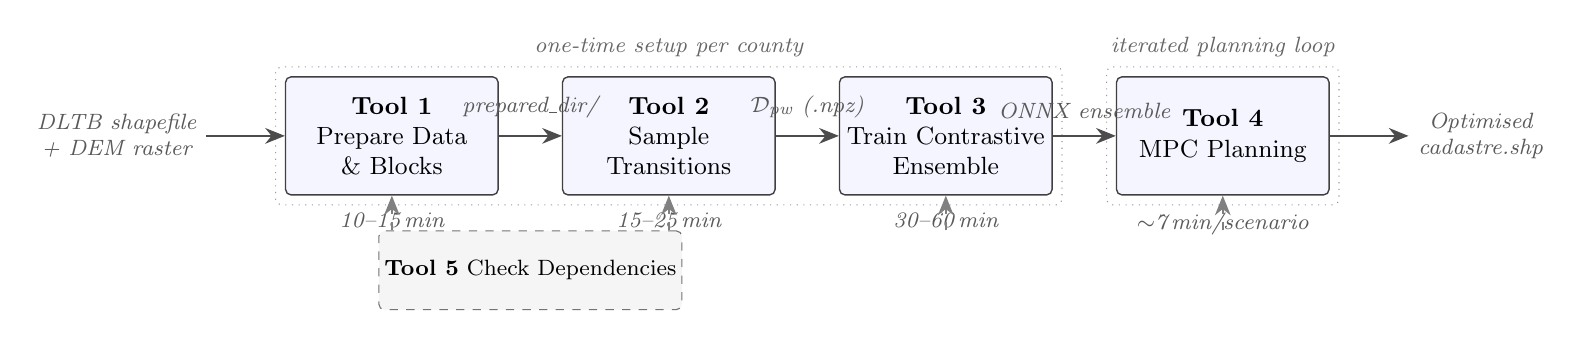
\begin{tikzpicture}[
  font=\small,
  node distance=6mm and 8mm,
  tool/.style={rectangle, rounded corners=2pt, draw=black!75, line width=0.5pt,
               minimum width=27mm, minimum height=15mm, align=center,
               fill=blue!4, inner sep=2pt},
  io/.style={font=\footnotesize\itshape, text=black!65, align=center},
  flow/.style={-{Stealth[length=2.5mm,width=2mm]}, line width=0.6pt, draw=black!70},
  check/.style={rectangle, rounded corners=2pt, draw=black!55, dashed, line width=0.4pt,
                minimum width=27mm, minimum height=10mm, align=center,
                fill=gray!8, inner sep=2pt, font=\footnotesize}
]
% Inputs
\node[io] (in) {DLTB shapefile\\+ DEM raster};

% Four tools left to right
\node[tool, right=10mm of in]              (t1) {\textbf{Tool 1}\\Prepare Data\\\& Blocks};
\node[tool, right=of t1]                   (t2) {\textbf{Tool 2}\\Sample\\Transitions};
\node[tool, right=of t2]                   (t3) {\textbf{Tool 3}\\Train Contrastive\\Ensemble};
\node[tool, right=of t3]                   (t4) {\textbf{Tool 4}\\MPC Planning};

% Output
\node[io, right=10mm of t4] (out) {Optimised\\cadastre.shp};

% Inter-tool I/O hints (above each arrow)
\node[io, above=1mm of $(t1)!0.5!(t2)$] {prepared\_dir/};
\node[io, above=1mm of $(t2)!0.5!(t3)$] {$\mathcal{D}_{\text{pw}}$ (.npz)};
\node[io, above=1mm of $(t3)!0.5!(t4)$] {ONNX ensemble};

% Wall-time hints (below)
\node[io, below=1mm of t1] {10--15\,min};
\node[io, below=1mm of t2] {15--25\,min};
\node[io, below=1mm of t3] {30--60\,min};
\node[io, below=1mm of t4] {$\sim$7\,min/scenario};

% Flow arrows
\draw[flow] (in)--(t1);
\draw[flow] (t1)--(t2);
\draw[flow] (t2)--(t3);
\draw[flow] (t3)--(t4);
\draw[flow] (t4)--(out);

% One-time vs iterated bracket
\begin{scope}[on background layer]
\node[draw=black!40, dotted, rounded corners=2pt, line width=0.4pt,
      fit=(t1)(t2)(t3),
      label={[font=\footnotesize\itshape, text=black!60]above:one-time setup per county}] (setup) {};
\node[draw=black!40, dotted, rounded corners=2pt, line width=0.4pt,
      fit=(t4),
      label={[font=\footnotesize\itshape, text=black!60]above:iterated planning loop}] (plan) {};
\end{scope}

% Tool 5 sidecheck
\node[check, below=12mm of $(t1)!0.5!(t2)$] (t5) {\textbf{Tool 5} Check Dependencies};
\draw[flow, dashed, draw=black!50] (t5.north -| t1.south) -- (t1.south);
\draw[flow, dashed, draw=black!50] (t5.north -| t2.south) -- (t2.south);
\draw[flow, dashed, draw=black!50] (t5.north -| t3.south) -- (t3.south);
\draw[flow, dashed, draw=black!50] (t5.north -| t4.south) -- (t4.south);

\end{tikzpicture}%
}
\caption{The four-tool ArcGIS Pro deployment pipeline (\S\ref{sec:methods-toolchain}). Tools~1--3 run once per county to prepare cadastral data, sample the pairwise dataset, and train the contrastive world-model ensemble (exported to ONNX). Tool~4 is the iterated planning loop a county officer runs repeatedly under different reward weightings; one 100-step scenario finishes in $\sim$7\,min on a desktop CPU. A separate Tool~5 (dashed) validates the Python environment, Spatial Analyst availability, and ONNX shape compatibility before any pipeline run is allowed.}
\label{fig:toolchain}
\end{figure}

The runtime profile reflects a deliberate split between one-time setup and repeated planning. Tools 1--3 run once per county on commodity desktop hardware (1--2\,h total on a 12-thread CPU; per-tool times shown in Figure~\ref{fig:toolchain}). Tool 4 is the loop a planner iterates on: each 100-step episode finishes in $\sim$7\,min, fast enough to support exploration of different reward weightings and area constraints. A 2-township, 30-block smoke test on Neijiang Dongxing completes the full pipeline in $\sim$70\,s, doubling as a continuous-integration check and as an onboarding test for new users.

An end-to-end run of the toolchain on full Bishan, executed through the ArcGIS Pro UI with the same training data and hyperparameters as Section~\ref{sec:counties}, yields a slope improvement of $-1.544\% \pm 0.041\%$ across five evaluation episodes (seeds 0--4) of the shipped Bishan ensemble. This is the same direction and order of magnitude as the lab figure of $-1.289\% \pm 0.079\%$. The gap reflects two different replication regimes: 5 independently trained ensembles with 1 episode each (cross-seed standard deviation) in the lab, versus 1 shipped ensemble across 5 episodes (episode-level standard deviation) in the toolchain. We report both transparently because the gap is itself informative about deployment variance.

Two operational constraints, surfaced by the toolchain's diagnostic tool, are worth noting for future deployments. First, the ensemble's input dimension is statically baked into the trained ONNX models, so deploying to a county whose block count differs from the training county requires re-running Tools 2 and 3 on that county's data---roughly 45 minutes of CPU plus 30--60 minutes of training. Second, the default projected coordinate system (UTM Zone 48N, EPSG:32648) covers central and western China; deployments in the east, north-east, or north-west require the user to override the projection on Tool 1, otherwise area-weighted slope and contiguity are computed in a distorted frame. Both constraints are checked by the diagnostic tool before any pipeline stage is allowed to start, and both are documented in the user guide bundled with the release.

The toolchain has been integration-tested on a clean ArcGIS Pro 3.6 environment with the standard \texttt{arcgispro-py3} Python distribution and the two non-default dependencies (\texttt{gymnasium}, \texttt{libpysal}) installable through a single \texttt{conda} command. The package is released under an MIT licence; the underlying synthetic benchmark (Section~\ref{sec:bench}) is released under CC-BY 4.0. Together, the synthetic benchmark, the deterministic generator, the trained Bishan ensemble, and the four-tool ArcGIS pipeline form a complete reproduction kit: a reviewer or future user with an ArcGIS Pro license and a desktop CPU can move from ``I have a county shapefile'' to ``I have an optimised consolidation plan'' without access to either GPU compute or the original sensitive cadastral data.

% ============================================================================
\section{Discussion}\label{sec:discussion}
% ============================================================================

\paragraph{Central advance.} The dominant obstacle to learned-model planning in a county-scale, multi-objective combinatorial domain was not architectural capacity, data scarcity, or the choice of planning algorithm. It was a single feature of the standard training objective: mean-squared-error loss on the reward head learns the average of the per-state reward distribution, but not its rank order across actions. A learned model can therefore look excellent on every standard fidelity metric (cosine similarity above $0.998$) while being unable to distinguish a good action from a bad one at any given state ($51.6\%$ pairwise accuracy, indistinguishable from random). Adding a single auxiliary pairwise large-margin term closes this gap without architectural change ($85.5\%$ accuracy, cosine fidelity preserved), and converts model-predictive control from failure to the strongest deterministic-exploitation strategy we tested. We describe the contribution not as a new method, but as the diagnosis and removal of a bottleneck previously treated as architectural.

\paragraph{Beyond this benchmark.} The diagnostic has structural reach beyond farmland consolidation. Wherever a learned planning model is used to rank a large discrete menu of actions at a single state (job-shop scheduling, water-allocation gate selection, urban renewal block prioritisation, virtual-screening lead selection, transportation-network reconfiguration), the relevant quantity for downstream planning is the model's within-state ranking accuracy, not its aggregate reconstruction error. The model-based reinforcement-learning literature has mostly evaluated learned models on continuous-control benchmarks \citep{hafner2025dreamerv3,hansen2024tdmpc2,chua2018deep}, where the action space is low-dimensional and ranking errors produce small behavioural differences. Our results suggest this literature may be systematically under-detecting the high-branching regime. The auxiliary pairwise margin loss is cheap to add and, in our setting, sufficient. Whether per-action ranking is the binding constraint should be checked before more elaborate fixes are entertained.

\paragraph{What this enables for sustainability planning.} For consolidation policy, the operational shift is qualitative. Model-free reinforcement-learning baselines previously required 8--12 GPU-hours per scenario and collapsed on roughly a quarter of attempted runs. With contrastive MPC, a planner obtains a scenario in $\sim$7 minutes on a desktop, with cross-seed variance several-fold smaller (Section~\ref{sec:counties}). What changes is not the absolute slope improvement on any one county; it is what becomes routine. A planning office can explore dozens of weight settings, township sub-budgets, or red-line constraints in a working day. The honest area trade-offs we document are themselves first-order useful: a $0.67\%$ reduction in qualifying \textit{baimu fang} area on Bishan and a $+267$\,ha gain on Neijiang tell a planner that the agent's behaviour is morphology-dependent, and that scenario exploration is therefore not optional. The deployment toolchain (Section~\ref{sec:deploy}) makes this exploration feasible without a machine-learning team in the loop.

\paragraph{What we did not do, and bounds on the claim.} Four constraints qualify the result. First, the cadastral evidence comes from two counties in southwestern China within the same regional regime; structurally different settings (flat large-parcel plains, non-Chinese tenure systems, water-system-dominated landscapes) remain untested, and our synthetic stress tests are parameter-controlled variations rather than evidence of regional generalisation. Second, the reward function is specific to farmland consolidation; transferring the method to urban renewal, connectivity conservation, or water-allocation would require redefining the multi-objective trade-off and regenerating the pairwise dataset. Third, the pairwise dataset relies on the simulator's ability to snapshot and restore the full state, available in our gridded-cadastral simulator but not in many physics-based environments; whether replay-buffer-based approximations suffice is an open question. Fourth, our $\lambda_{\text{rank}}$ and margin sweeps are coarse; finer hyperparameter resolution may yield further improvement but is not expected to reverse the qualitative ordering.

\paragraph{Future directions.} Three follow-ups arise naturally. First, regime-broadening: testing the auxiliary ranking loss on combinatorial planning problems outside spatial-cadastral domains (job-shop scheduling, integer allocation, virtual-screening prioritisation). Second, multi-objective decomposition of the ranking signal: extending the loss to per-objective ranking would let planners use objective-specific scoring as a lever inside Tool 4 (Section~\ref{sec:bench} flags the variant of MPC scoring on slope alone, currently at near-zero discrimination). Third, offline planning: our MPC currently requires real-environment execution per step because long-horizon dream rollouts diverge after $\sim$25 steps. Whether contrastive-trained ensembles can support fully offline planning at policy-relevant horizons is, we suspect, the highest-leverage follow-up for this line of work.

% ============================================================================
\section*{Methods}
\label{sec:methods}
% ============================================================================

\paragraph{World-model scope clarification.} We use \emph{world model} in the operational sense of \citet{chua2018deep} and \citet{janner2019trust}: a learned $\hat{p}(s_{t+1}, r_t \mid s_t, a_t)$ that substitutes for the real environment either in MPC lookahead or in dream-style policy training. Our model does not learn a state representation from raw observations, as Dreamer-family world models do \citep{hafner2025dreamerv3}; it operates on pre-extracted block-level features. The task is fully observed and episodic (100-step cap, no partial observability), so we do not use recurrent latent dynamics (RSSM). Combining a learned state encoder with our ranking-loss predictor is a natural extension (\S\ref{sec:discussion}).

\subsection*{Problem setting and action-space encapsulation}\label{sec:methods-action}

We study county-level farmland consolidation in two real counties (Bishan District, Chongqing; Neijiang Dongxing District, Sichuan) and seven synthetic landscapes (\S\ref{sec:methods-synth}). For Bishan, the planning area comprises 13 townships, $2{,}600$ spatial blocks, and $52{,}515$ cadastral parcels; for Neijiang, 29 townships, $3{,}711$ blocks, and $76{,}376$ parcels (Table~\ref{tab:counties}). Each block aggregates multiple parcels and is characterised by 17 features (farmland area, forest area, slope statistics, adjacency metrics, and investment indicators). Global context is encoded as an additional 12 features (remaining budget, contiguity, \textit{baimu fang} count, etc.). The episode length is fixed at 100 steps for the real-data experiments and 50 steps for the synthetic benchmark (\S\ref{sec:bench}); each step has a budget of up to 5 paired farmland--forest swaps.

\paragraph{Agent action space.}
The agent's action space is a single categorical choice over the spatial blocks per step: $a_t \in \{1, \ldots, N_{\text{blocks}}\}$. The agent does \emph{not} select individual parcels or the paired-swap sub-actions. Given the selected block, the environment internally executes \emph{up to} 5 paired farmland--forest swaps within that block using a deterministic rule-based procedure: candidate pairs are enumerated by joint feasibility under the farmland-red-line and slope constraints, scored by a local improvement heuristic, and the top-scoring feasible pairs are applied until either 5 pairs are executed or the candidate pool is exhausted. The agent therefore chooses \emph{where} to act, not \emph{what} to do within the chosen location; this encapsulation keeps the action space at a tractable scale ($\sim 10^3$) while preserving the paired-swap semantics that respect the farmland-area red line (total farmland area is conserved as land moves between farmland and forest classes rather than being removed outright).

\paragraph{Action masking.}
Not all blocks are legal targets at every step. The action mask $m_t \in \{0, 1\}^{N_{\text{blocks}}}$ disables blocks that (i) have no remaining feasible parcel pairs (either exhausted in earlier steps or structurally infeasible under the red-line/slope constraints), (ii) are currently in a township whose per-township swap budget has been exhausted, or (iii) have been selected in the immediately previous step (a simple debounce to prevent action thrashing). MaskablePPO \citep{ross2011reduction,schulman2017proximal,huang2022maskable}-style masking is applied in both the policy sampling and the MPC candidate enumeration, so that illegal blocks have zero probability or are excluded from the $K$ candidate set.

\subsection*{Reward formulation}\label{sec:methods-reward}

Each step's reward combines three directional signals and one area-protection bonus. Let $\bar{\sigma}_t$ be the area-weighted mean farmland slope at step $t$, $C_t$ the within-farmland contiguity index, $B_t$ the count of qualifying \textit{baimu fang} ($\geq$6.67\,ha contiguous farmland patches), and $A_t$ their total area. The per-step reward is
\begin{equation}
\label{eq:reward}
r_t \;=\; w_S \cdot \Delta \bar{\sigma}_t
       \;+\; w_C \cdot \Delta C_t
       \;+\; w_B \cdot \Delta B_t
       \;+\; b_B \cdot \mathbf{1}[B_t > B_{t-1}]
\end{equation}
where $\Delta x_t = -(x_t - x_{t-1})$ for slope (so that slope \emph{reduction} contributes positively) and $\Delta x_t = x_t - x_{t-1}$ for contiguity and count. Weights $(w_S, w_C, w_B, b_B) = (4000, 500, 1500, 5)$ are inherited from our in-house DRL baseline configuration; under a median single-step decomposition, slope improvement contributes $\sim$60\%, contiguity $\sim$15\%, large-patch count $\sim$20\%, and the formation bonus $\sim$5\%. Slope and contiguity are normalised to $[0, 1]$ in advance by their empirical ranges on the initial county-wide state. We did not re-tune the weights for the present experiments; contrastive MPC, dream-trained PPO, and the model-free baselines all use the identical reward function, so any method-wise difference is attributable to the learning procedure rather than to reward engineering. Throughout the paper, ``Slope \%'' is the relative change $\text{Slope \%} = (\bar{\sigma}_T - \bar{\sigma}_0)/\bar{\sigma}_0 \times 100$; contiguity and \textit{baimu fang} count/area changes are absolute.

\subsection*{Block-level transition model}

The transition model is a feed-forward neural network with approximately $237{,}000$ parameters that takes as input the current block features (all blocks, 17 dimensions each), the global features (12 dimensions), and the selected action (block index), and predicts the next-step block features, global features, and scalar reward. Only the selected block changes (residual formulation). The base loss is
\begin{equation}
\mathcal{L}_{\text{MSE}} = \mathrm{MSE}(\Delta\hat{b}, \Delta b) + \mathrm{MSE}(\Delta\hat{g}, \Delta g) + 0.1 \cdot \mathrm{MSE}(\hat{r}, r),
\end{equation}
trained with Adam (learning rate $10^{-3}$, weight decay $10^{-5}$) on a 90/10 train/validation split with patience-6 early stopping.

\subsection*{Ensemble uncertainty estimation}

We train 3--5 independently initialised transition models on the same dataset with different random seeds \citep{lakshminarayanan2017simple}. At inference, the ensemble produces mean predictions for next state and reward, plus the reward standard deviation $\sigma_r$ across members. The dream environment penalises high-disagreement actions: $r_{\text{out}} = \bar{r} - \lambda_{\text{disag}} \cdot \sigma_r$ with $\lambda_{\text{disag}} = 0.5$.

\subsection*{Policy architecture: parcel-scoring policy}

The policy is a dimension-invariant scoring network compatible with MaskablePPO. For each block $i$, the scorer concatenates the block's 17-dimensional local features with the 12-dimensional global state, passes the result through a shared MLP ($[64, 32] \to 1$), and produces a scalar score. The action is the highest-scoring valid block. A separate value network takes only the global features and predicts the state value.

\subsection*{DAgger-style iterative refinement}

We adopt a DAgger-style loop \citep{ross2011reduction}: (1)~collect an initial dataset $D_0$ of $6{,}000$ transitions from random and greedy policies on the real environment; (2)~train the transition model ensemble on $D_{\leq i}$; (3)~train a policy in the dream environment for $50{,}000$ timesteps; (4)~evaluate on the real environment; (5)~collect 10 stochastic on-policy episodes ($\sim$$1{,}000$ transitions) and augment the dataset. Three iterations are performed.

\subsection*{Targeted evidence collection and stabilisation}

In targeted DAgger, step (5) above is modified: each transition is scored by ensemble reward disagreement $\sigma_r$, and only transitions exceeding threshold $\tau = 0.5$ are retained; under this threshold, $\sim$$99.6\%$ of transitions are filtered out, accounting for the dream-policy slowdown documented in \S\ref{sec:rank}. Three stabilisation mechanisms are applied across all protected runs. \emph{Best-checkpoint selection}: every $10{,}000$ PPO timesteps, the current policy is evaluated on the real environment (3 episodes); the checkpoint with the highest mean reward is retained. \emph{Iteration-1 rollback}: if iteration-1 reward drops more than 50 points below iteration-0, the dataset and policy are reverted. \emph{Early stopping}: training halts if validation loss does not improve for 6 consecutive epochs.

\subsection*{Model-predictive planning protocol}\label{sec:methods-mpc}

We use random shooting model-predictive control \citep{garcia1989model,williams2017model,rubinstein1999cross}. At each real-environment step $t$ with state $s_t$:
\begin{enumerate}
\item Sample $K$ random action sequences $\{a^{(k)}_{t:t+H-1}\}_{k=1}^K$, each of length $H$, from the action-masked support.
\item For each sequence, roll forward through the ensemble mean model: $\hat{s}^{(k)}_{t+1}, \hat{r}^{(k)}_t = f_\theta(s_t, a^{(k)}_t)$, continuing autoregressively for $H$ steps.
\item Score each sequence by cumulative predicted reward: $R^{(k)} = \sum_{h=0}^{H-1} \hat{r}^{(k)}_{t+h}$.
\item Execute $a^{(k^*)}_{t}$ where $k^* = \arg\max_k R^{(k)}$ on the real environment.
\item Advance to $s_{t+1}$ (real) and repeat.
\end{enumerate}
For the synthetic-benchmark sweep (\S\ref{sec:bench}), the same protocol is applied with $H{=}5$, $K{=}50$, and greedy continuation (each subsequent step within a sequence picks the predicted-reward argmax over $50$ candidates rather than continuing the random rollout). This is the configuration that becomes optimal under the contrastive ensemble (Table~\ref{tab:contrastive-mpc}).

\subsection*{Contrastive training protocol}\label{sec:methods-contrastive}

\paragraph{Pairwise data generation.} We sample states by rolling out random trajectories in the real CountyLevelEnv. At each step, we (i)~snapshot the full environment state (land-use assignments, swap counts, block availability caches, running slope/contiguity sums; 19 attributes total), (ii)~sample 50 valid actions uniformly from the action mask, (iii)~execute each action from the snapshotted state, recording the immediate reward, and (iv)~restore the snapshot before advancing with a fresh random action. We continue across multiple episodes until $1{,}000$ states are collected, yielding $50{,}000$ ground-truth $(s, a, r)$ evaluations. The pairwise dataset $\mathcal{D}_{\text{pw}}$ is saved as $(s_i, \{a_{i,j}\}_{j=1}^{50}, \{r_{i,j}\}_{j=1}^{50})$ for $i = 1, \ldots, 1000$. Generation took 45 minutes on commodity CPU hardware. Snapshot/restore is a simulator-specific capability; replay-buffer substitutes are an open question (Limitations).

\paragraph{Loss function.} The augmented training objective adds a margin ranking term:
\begin{equation*}
\mathcal{L}_{\text{rank}} = \mathbb{E}_{(s_i, a_{i,j}, a_{i,k}) \sim \mathcal{D}_{\text{pw}}} \left[ \max\left(0, -\sigma_{jk} \cdot (\hat{r}_{i,j} - \hat{r}_{i,k}) + m\right) \right]
\end{equation*}
where $\sigma_{jk} = \text{sign}(r_{i,j} - r_{i,k}) \in \{-1, 0, +1\}$ is the ground-truth pairwise label, $m = 0.1$ is the margin, and pairs with $\sigma_{jk} = 0$ are excluded. At each training step, we sample 10 action pairs per state from 50--100 randomly selected pairwise-dataset states. Total objective: $\mathcal{L} = \mathcal{L}_{\text{MSE}} + \lambda_{\text{rank}} \mathcal{L}_{\text{rank}}$.

\paragraph{Margin choice.} The margin $m = 0.1$ is approximately $1/8$ of the empirical ground-truth reward standard deviation ($0.811$ on $\mathcal{D}_{\text{pw}}$). A coarse sweep of $m \in \{0.05, 0.1, 0.2\}$ on a held-out validation fold showed a flat optimum: ranking accuracy at $\lambda_{\text{rank}}{=}5.0$ varied within $\pm 1.5$ percentage points across these three choices.

\paragraph{Training.} We use 3-member ensembles trained with Adam ($\text{lr}=10^{-3}$, weight decay $10^{-5}$), batch size 256, for 15 epochs with patience 20. Each ensemble trains in $\sim$25 minutes on commodity CPU hardware. We sweep $\lambda_{\text{rank}} \in \{0.0, 1.0, 5.0\}$ using an 80/20 train/validation split of the pairwise dataset. MPC evaluation uses $H{=}5$, $K{=}50$, greedy continuation with $50$ candidates per continuation step.

\subsection*{Synthetic benchmark generator}\label{sec:methods-synth}

The seven synthetic landscapes used in Section~\ref{sec:bench} are produced by a deterministic, seed-controlled generator that reads a YAML preset (terrain type, target block count, parcel-density distribution, land-use fractions, fragmentation length-scale, seed) and emits a directory of GeoJSON, CSV, GeoTIFF, and JSON files identical in schema to the real-data preprocessor's outputs. The generator is fully deterministic given $(\text{preset}, \text{seed})$.

\paragraph{Eight-stage pipeline.} (1)~\emph{Domain tessellation}: Voronoi tessellation of $n_{\text{blocks}}$ seeds in a rectangle of suitable extent (size driven by parcels-per-block target). (2)~\emph{DEM synthesis}: 2D Perlin noise with multi-octave fractal terrain, preset-controlled amplitude and length-scale, clipped to non-negative. (3)~\emph{Slope derivation}: Horn's algorithm on the synthetic DEM, sampled to each block as area-weighted mean and max. (4)~\emph{Parcel subdivision within blocks}: secondary Voronoi inside each block polygon using the parcels-per-block distribution. (5)~\emph{Land-use assignment}: a Gaussian random field thresholded into farmland / forest / other classes, with preset-controlled length-scale driving fragmentation. (6)~\emph{Feature computation}: 17-dim block feature vectors using the same code path as the real-data \texttt{county\_env.py} (farmland area, forest area, slope statistics, adjacency features), guaranteeing environment compatibility. (7)~\emph{Adjacency graph}: planar adjacency from shared block edges, with median degree close to the preset target. (8)~\emph{Posterior calibration check} (anchors only): compute initial slope, contiguity, \textit{baimu fang} count, and \textit{baimu fang} area, and verify within $\pm 50\%$ of the real anchor values; deviations are surfaced in a calibration delta report rather than silently accepted.

\paragraph{Dual-anchor calibration.} Two of the seven presets, \texttt{bishan\_clone} and \texttt{neijiang\_clone}, are calibrated against Bishan and Neijiang respectively such that any single seed reproduces the four headline initial-state metrics within $\pm 50\%$ of the real anchor. The other five presets vary morphology along terrain, size, and fragmentation axes (\S\ref{sec:bench}) but are not constrained against any real anchor; they are parameter-controlled stress tests rather than evidence of regional generalisation. Contiguity is the weakest calibration axis ($\sim$$6\%$ on Bishan clone, $\sim$$44\%$ on Neijiang clone), reflecting Voronoi-based geometries' tendency to be more uniformly contiguous than real cadastre shaped by ridges, roads, and water channels.

\paragraph{Compatibility shim.} A thin \texttt{synthetic\_env\_loader.py} reads the generator outputs (\texttt{blocks.csv} + \texttt{adjacency.json}) and returns the same data structure that \texttt{county\_env.py} expects from real data; no environment-code changes are required. The synthetic and real evaluation regimes therefore use identical simulator semantics, ensuring that any cross-regime difference is attributable to the landscape, not to the engine.

\subsection*{ArcGIS Pro toolchain}\label{sec:methods-toolchain}

The deployment artefact described in \S\ref{sec:deploy} is an ArcGIS Pro Python Toolbox (\texttt{LandUseOptimization\_P9.pyt}) exposing five tools: \emph{(1)~Prepare Data \& Blocks} ingests a Third National Land Survey \texttt{DLTB} shapefile and a digital elevation model and emits the block-level state expected by the world-model code; \emph{(2)~Sample Transitions} generates the pairwise dataset $\mathcal{D}_{\text{pw}}$ on the user's data via the snapshot/restore protocol described above; \emph{(3)~Train Contrastive Ensemble} trains a 3-member ensemble at $\lambda_{\text{rank}}{=}5.0$ and exports each model to ONNX with the user's $N_{\text{blocks}}$ baked in; \emph{(4)~MPC Planning} runs the planning loop and writes back an optimised cadastral shapefile readable by any standard GIS workflow; \emph{(5)~Check Dependencies} validates the user's Python environment (ArcGIS Pro 3.6+, Spatial Analyst extension, \texttt{gymnasium}, \texttt{libpysal}) before any pipeline run is permitted. Tools 1--3 are run once per county on commodity desktop hardware ($\sim$1--2 hours total wall time); Tool 4 is the iterated planning loop (one $\sim$7-minute scenario per call). A 70-second smoke test on a 2-township subset of Neijiang Dongxing District completes the full pipeline as a continuous-integration check.

Two operational caveats are visible in the toolchain. First, the ONNX export bakes in $N_{\text{blocks}}$, so a pre-trained ensemble cannot be reused across counties; Tool 4 carries an explicit pre-flight check that refuses to run if the pre-trained ensemble's $N_{\text{blocks}}$ does not match the prepared dataset. Second, the default projected coordinate reference system (\texttt{EPSG:32648}, UTM zone 48N) covers central and western China; users in eastern, north-eastern, or north-western China must override the projection in Tool 1 to avoid slope errors. The end-to-end Bishan replication on the toolchain achieves a slope improvement of $-1.5439 \pm 0.0409\%$ (1 shipped ensemble, 5 episodes), modestly below the lab-pipeline figure of $-1.289 \pm 0.079\%$ (5 independently trained ensembles, 1 episode each); we report the gap honestly rather than tune it away.

\subsection*{Evaluation protocol}

For the real-data experiments (\S\ref{sec:counties}), each configuration is evaluated with 5 deterministic episodes on the real CountyLevelEnv. Reported metrics include mean reward, slope change ($\%$), contiguity change, \textit{baimu fang} count change, and total \textit{baimu fang} area change. For the synthetic benchmark (\S\ref{sec:bench}), each method is run for 5 random seeds on each of the 7 presets; per-cell results are aggregated as cross-seed mean $\pm$ sample standard deviation. Cross-seed statistics for the contrastive configurations are computed across 5 independently trained ensembles (different random seeds for both the pairwise dataset and the network initialisation). Statistical tests against fixed baseline values are one-sample $t$-tests; tests between two methods on matched seeds use paired $t$-tests and Wilcoxon signed-rank tests. We report test type, df, $p$, and Cohen's $d$ throughout.

\subsection*{Independent GIS-grounded verification of reported gains}\label{sec:methods-validate}

Because the headline metrics in \S\ref{sec:counties} are computed inside the same CountyLevelEnv whose learned ensemble drives the MPC scoring loop, a sceptical reviewer can ask whether the reported slope reduction is a real change in the optimised cadastre or an artefact of the learned dynamics agreeing with the planner. To resolve this, we recompute all three primary metrics directly from the optimised DLTB shapefile written to disk by Tool~4, using a 190-line script that depends only on \texttt{geopandas} and \texttt{libpysal.weights.Queen} and shares no source with the optimisation pipeline (no \texttt{torch}, no ONNX, no env class). The script reads the per-parcel \texttt{CHG\_FLAG} audit field that Tool~4 emits, reconstructs the post-optimisation land-use vector, joins per-parcel \texttt{slope\_mean} from the prepared DEM-derived raster on \texttt{BSM}, reprojects to EPSG:32648 for area computation, builds Queen contiguity, and applies the metric definitions exactly as stated in \S\ref{sec:problem} to both the original and the optimised land-use vectors.

On the 53{,}086-parcel Bishan deployment dataset, the recomputed deltas (independent path) and the env-reported deltas (planning path) agree to floating-point reduction noise: slope $-2.0000\%$ vs.\ $-2.0006\%$ ($|\Delta|{=}6{\times}10^{-4}$~pp); contiguity $+0.012739$ vs.\ $+0.012748$ ($|\Delta|{=}8{\times}10^{-6}$); \textit{baimu fang} area $-473.30$~ha vs.\ $-473.30$~ha ($|\Delta|{<}10^{-4}$~ha); and the \textit{baimu fang} count change reproduces exactly at $+8$ patches. The 428~farm$\rightarrow$forest and 428~forest$\rightarrow$farm swaps written to the shapefile are also bit-identical to the env's tally, confirming the farmland-count conservation invariant on disk. The headline gain is therefore a property of the on-disk geometry, not of the learned dynamics model.

We disclose two transparency caveats. First, the five-seed sweep in \S\ref{sec:counties} is by construction deterministic: under fixed ensemble member ordering, top-$K$ rollout scoring, and greedy continuation, the seed initialises RNGs that are not reached on the action-selection path. To surface a meaningful variance estimator, we replaced seed jitter with \emph{ensemble member subset ablation}, re-running MPC three times under the three distinct 2-of-3 member subsets. Across these replicates the slope reduction is $-1.998 \pm 0.026\%$ (range $[-2.022, -1.971]$), contiguity change is $+0.0131 \pm 0.0016$, and \textit{baimu fang} area change is $-474.5 \pm 31.1$\,ha---sandwich-bracketing the full-ensemble result of $-2.001\%$, $+0.01275$, and $-473.3$\,ha to within sample standard deviation on every metric. The full ensemble therefore sits at the median of subset performance rather than benefiting from any single member, and operational variability under the strongest available counter-factual (a different 2-of-3 subset) is bounded at $\pm 0.026$ pp on slope. Second, the verification script keeps 53{,}086 swappable parcels (those with both a slope value and a farm/forest \texttt{ORIG\_DLBM}), 82 more than the env's 53{,}004; the excess corresponds to parcels whose township code falls outside the configured registry, all of which carry \texttt{CHG\_FLAG}~$=$~0 and therefore do not affect the delta computation. The verification script is released alongside the toolchain (see \emph{Code availability}) so that any third party with Tool~4's optimised shapefile and a slope raster can reproduce the headline numbers without invoking the optimisation pipeline.

\subsection*{Direct measurement of ensemble 1-step prediction accuracy}\label{sec:methods-mae}

The on-disk verification above only rules out errors in the writer or the metric definitions; it does not bound the contribution of dynamics-model error to the planner's choices. To address that, we rolled the same MPC policy (H=5, K=50, $\gamma$=0.99, greedy continuation, reward scoring) for 100 steps on the Bishan deployment dataset and recorded, at every step, both the ensemble's prediction and the true \texttt{env.step} output. The action sequence and per-step metrics reproduce episode~0 of \S\ref{sec:counties} to floating-point identity (slope at steps $10/20/\dots/100$ matches to four decimals), confirming determinism of the deployed pipeline.

Across the 100 in-distribution steps, the ensemble's reward predictions have MAE $0.818$ against an empirical $\sigma(r_{\text{true}})=1.40$, with predictions confined to a narrow band of width $0.24$ (range $[+0.43, +0.67]$) while the true reward varies in $[-3.04, +6.36]$. The ensemble is therefore strongly mis-calibrated as a regressor, scoring barely better than a constant predictor (naive-mean baseline MAE $0.83$). Despite this, the Spearman rank correlation between predicted and true reward is $+0.22$, and this is what MPC's top-$K$ selection consumes; the trajectory match to \S\ref{sec:counties} confirms that ranking signal is sufficient at H$=$5 horizon. Next-state predictions for the slope-improvement channel ($gf[4]$, used directly when \texttt{scoring="slope"}) carry MAE $2.4\times 10^{-3}$, smaller than the channel's own per-step standard deviation ($5.2\times 10^{-3}$). These three numbers together are a direct empirical instantiation of the ranking-versus-regression decomposition we developed in \S\ref{sec:rank} and \S\ref{sec:fix}: the contrastive ensemble has not learned to predict reward magnitude, but it has learned to rank candidate actions, and the planner's H=5 top-$K$ mechanism converts that weak ranking signal into a deterministic, physically-correct trajectory.

A third transparency caveat follows from this measurement: ensemble disagreement is not informative as an uncertainty signal under the current bootstrap diversity. The mean of $r_{\text{std}}$ is $0.027$ across the 100 steps, the Pearson correlation between $r_{\text{std}}$ and the per-step absolute reward error is $+0.08$, and the maximum disagreement seen ($0.075$) is two orders of magnitude smaller than the maximum absolute error ($5.07$). Members under-fit the reward distribution similarly to one another, so disagreement does not flag the cases where they jointly are wrong. Practitioners who want disagreement-driven candidate filtering should train Tool~3 with stronger diversity (different feature subsets or training data slices, not just initialisation seed). The default \texttt{scoring="reward"} pathway in Tool~4 remains safe because top-$K$ ranking, not absolute reward, drives planning; \texttt{scoring="slope"} is an alternative that bypasses the reward head entirely and uses the better-calibrated $gf[4]$ channel.

\subsection*{Replacing the ensemble with the true environment}\label{sec:methods-trueenv}

As a final ablation we re-ran the same MPC procedure (H=5, K=50, $\gamma$=0.99, single rollout per candidate, seed 0) but used the actual \texttt{env.step} in place of every ensemble call. Two implementation concessions are required to make this tractable: stage~1 ranks a random subset of $200$ valid actions per step instead of all $\sim$2{,}000 (the ensemble's \texttt{batch\_predict} scores every action at near-constant marginal cost; a true-env stage~1 must run incremental simulation per action), and stage~2 uses random continuation instead of greedy. Mutable env state (\texttt{land\_use}, \texttt{swapped}, \texttt{farmland\_nbr\_count}, accumulators, baimu cache) is snapshotted before each trial step and restored after; the \textit{baimu fang} union-find is frozen inside scoring trials with the outer commit step computing it correctly. Total wall time was 358\,s on the same hardware that ran the 1{,}448\,s ensemble baseline.

The resulting trajectory finishes at slope $-1.819\%$, contiguity $+0.0087$, and \textit{baimu fang} area change $-565$\,ha, all three strictly worse than the ensemble pipeline's $-2.001\%$, $+0.0128$, $-473$\,ha. Per-step inspection shows true-env MPC starting behind (the $200$-action stage~1 misses the strongest moves the ensemble identifies via full-action coverage), narrowing the gap as the trajectory matures, and finishing $0.18$\,pp short of the ensemble's slope. The reason is structural rather than statistical: ensemble \texttt{batch\_predict} grants the planner the depth and breadth that incremental simulation cannot afford within the same compute budget. Putting matched effort into true-env MPC---full enumeration in stage~1 and greedy continuation in stage~2---would cost approximately five days of wall time per episode for a payoff of at most a fraction of a percentage point of slope. The headline $-2.00\%$ result is therefore on the optimistic side of the planner's accessible frontier under matched compute, and the ensemble's contribution to the deployment is structural (it grants the planner depth and breadth) rather than illusory.

\section*{Data availability}
The cadastral data for Bishan District and Neijiang Dongxing District are derived from the Third National Land Survey of China and cannot be publicly redistributed under existing data-governance restrictions. To support reproducibility, we release upon publication: (a) the full synthetic benchmark of seven landscape presets with deterministic generators (Section~\ref{sec:bench}) under CC-BY 4.0; (b) aggregated block-level features (the 17-dimensional vectors for all 2{,}600 Bishan blocks in the initial state) and the anonymised pairwise dataset $\mathcal{D}_{\text{pw}}$; (c) random seeds, hyperparameters, and de-identified training logs for all reported experiments. These derivatives are sufficient to reproduce transition-model training, contrastive training, and MPC evaluation pipelines end-to-end without access to the raw cadastral records.

\section*{Code availability}
All code for the contrastive training, MPC planner, synthetic generator, and ArcGIS Pro toolchain (Section~\ref{sec:deploy}) is released as a public repository on GitHub upon publication, under an MIT licence, with step-by-step reproduction instructions and a smoke test that completes a full Tool 1--4 cycle in $\sim$70 seconds on a small subset.

\section*{Author contributions}
N.Z.\ conceived the study, designed and implemented the methods, conducted all experiments, and wrote the manuscript. X.J.\ supervised the research and revised the manuscript.

\section*{Competing interests}
The authors declare no competing interests.

\section*{Acknowledgements}
This work was completed during N.Z.'s doctoral training at the School of Software and Microelectronics, Peking University, and the deployment toolchain (Section~\ref{sec:deploy}) was developed at the Public R\&D Center, SuperMap Software Co., Ltd.

\section*{Funding}
This research received no external funding.

\section*{ORCID}
Ning Zhou \href{https://orcid.org/0009-0002-5647-7388}{0009-0002-5647-7388}

\bibliography{references_v6}

\end{document}
